% 原始嵌入网络图完整保留全部节点、边和箭头；中文节点标签由 TikZ 排印。
\begin{figure}[htbp]
\centering
\begin{tikzpicture}[x=0.1044mm,y=-0.1044mm,inner sep=0pt]
\node[anchor=north west] (ch01dfig17data) at (0,0) {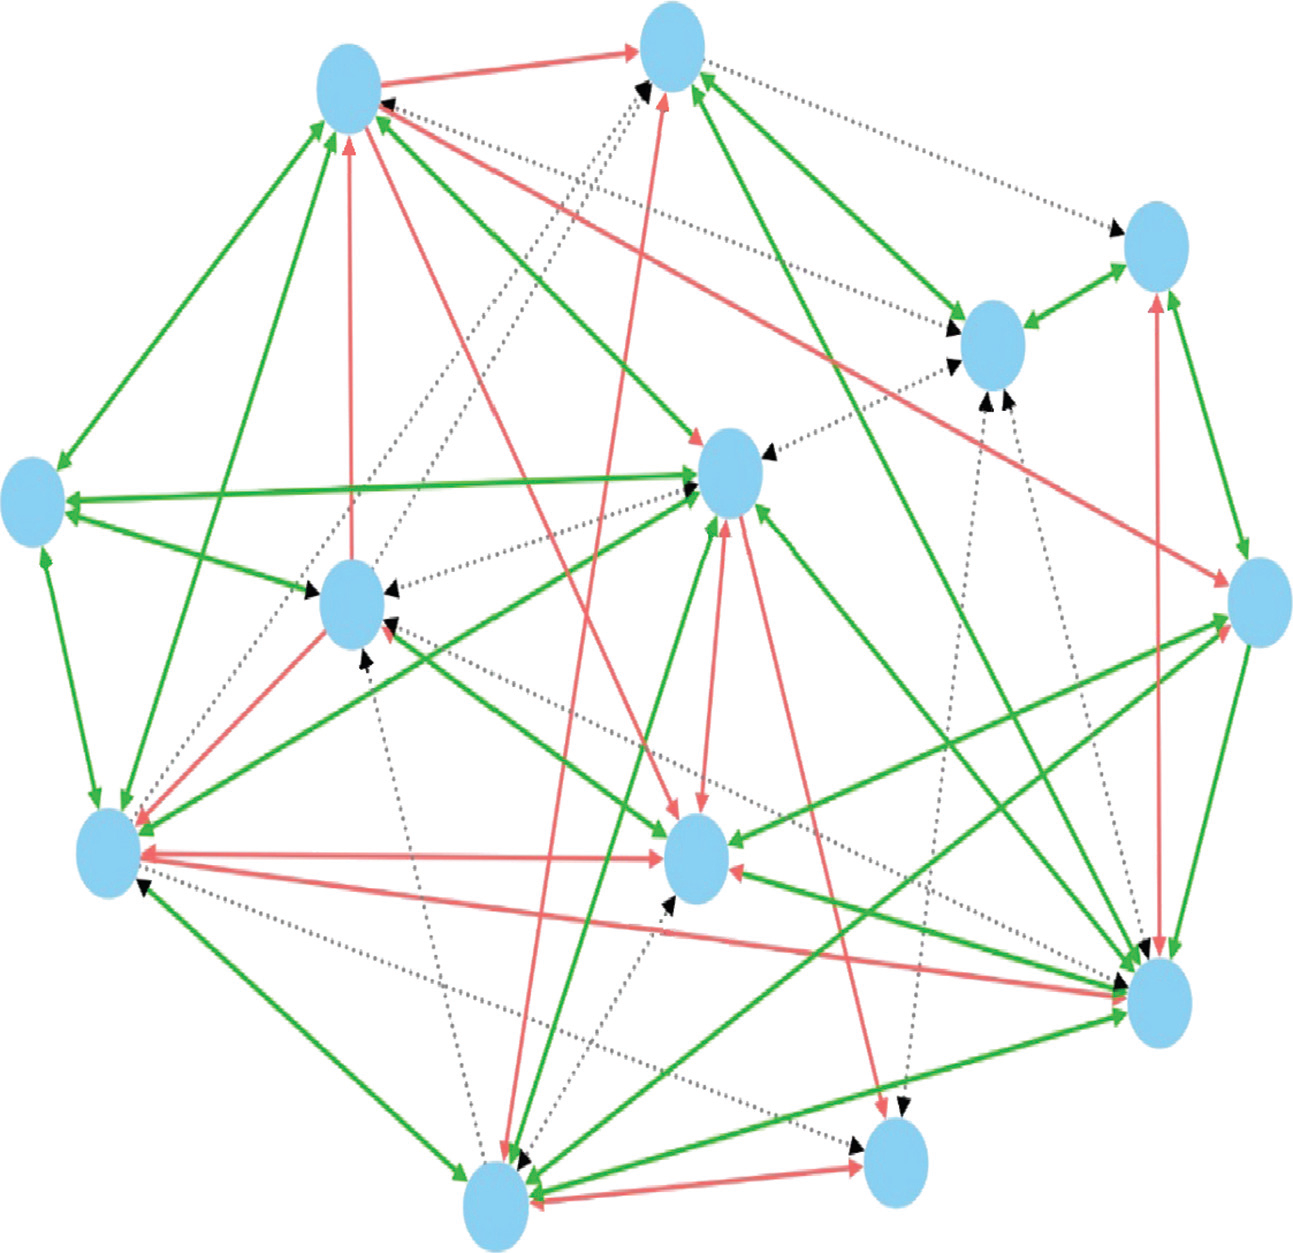
\includegraphics[width=135mm]{figures/ch01d_figure17_data.png}};
\node[fill=white,inner sep=0.5pt,font=\fontsize{8}{9}\selectfont] at (1162.487,1070.911) {WHR};
\node[fill=white,inner sep=0.5pt,font=\fontsize{8}{9}\selectfont] at (1286.196,669.837) {舒张压};
\node[fill=white,inner sep=0.5pt,font=\fontsize{8}{9}\selectfont] at (896.109,1229.734) {胆红素};
\node[fill=white,inner sep=0.5pt,font=\fontsize{8}{9}\selectfont] at (493.433,1274.677) {BMI};
\node[fill=white,inner sep=0.5pt,font=\fontsize{8}{9}\selectfont] at (106.990,925.282) {HDL};
\node[fill=white,inner sep=0.5pt,font=\fontsize{8}{9}\selectfont] at (717.845,927.522) {收缩压};
\node[fill=white,inner sep=0.5pt,font=\fontsize{8}{9}\selectfont] at (336.837,673.622) {血糖};
\node[fill=white,inner sep=0.5pt,font=\fontsize{8}{9}\selectfont] at (65.049,571.385) {总胆固醇};
\node[fill=white,inner sep=0.5pt,font=\fontsize{8}{9}\selectfont] at (741.064,541.052) {甘油三酯};
\node[fill=white,inner sep=0.5pt,font=\fontsize{8}{9}\selectfont] at (1016.175,418.600) {肌酐};
\node[fill=white,inner sep=0.5pt,font=\fontsize{8}{9}\selectfont] at (676.753,120.881) {尿素};
\node[fill=white,inner sep=0.5pt,font=\fontsize{8}{9}\selectfont] at (357.418,162.446) {LDL};
\node[fill=white,inner sep=0.5pt,font=\fontsize{8}{9}\selectfont] at (1184.078,312.995) {心率};
\end{tikzpicture}
\origfig{17}{从 UK-10K 和泰州队列数据集中识别出的两个表型网络，均包含 13 个节点和 54 条边。}
\label{fig:omics-real-phenotype-networks}
\end{figure}
